% \newpage
\subsection{Prototype 3}
\label{sub:prototype_3}

\subsubsection{Presentation}
\textbf{Tools:} proto.io

\paragraph{Rationale}

This prototype is based on the `flat' design of other booking apps. The search
criteria is spread across a number of pages and results are displayed as a
list.

\paragraph{Home Screen}
\marginpar{%
	\begin{overpic}[width=\marginparwidth]
		{img/firstPrototypes/Pro3Main}
	\end{overpic}
	\captionof{figure}{Home screen is also the search page}\label{fig:Pro3Home}
}

The home screen is also a search page. Users are able to search by sport,
location, distance, date and time or a combination of these options; all of
these have the default value of `Any' if the user decides not to enter a
specific value or range.

By selecting a search option, such as `sport', the user will be directed to
another page where they can specify a sport or combination of sports using a
checklist interface similar to the previous prototypes. The `date' section
would allow the user to select a specific date, a variety of dates or between
two dates using a calendar interface. The user can select a time-frame. E.g.
after 5pm, before 12pm or between 4pm and 8pm using the `time page'. Distance
can also be selected by range (e.g.\ up to 5 miles). Location can be selected
from a drop-down list of cities, the user can also type their location or use
GPS for their current location.

Once the user has selected their options they can use the `Search' button to
see their results.

\paragraph{Details}
\marginpar{%
	\begin{overpic}[width=\marginparwidth]
		{img/firstPrototypes/Pro3Details}
	\end{overpic}
	\captionof{figure}{Details screen}\label{fig:Pro3Details}
}

The `Details' button in the navigation bar can store information about the user
such as their age, which can help them to find offers that are relevant to them
or discounts can be applied to the price during the search.

Basic information about the user can be stored locally to apply discounts and
include relevant offers.

\paragraph{Results}
% \marginpar{%
% 	\begin{overpic}[width=\marginparwidth]
% 		{img/firstPrototypes/Pro3Results_1}
% 	\end{overpic}
% 	\captionof{figure}{Results displayed as a list}\label{fig:Pro3Results_1}
% }

The results page allows the user to see their search criteria as well as a list
of available facilities. These can be sorted by price or distance.

The user can go back to change the search criteria using the `Back' button on
the navigation bar or select one of the results in the list for more
information.
% \marginpar{%
% 	\begin{overpic}[width=\marginparwidth]
% 		{img/firstPrototypes/Pro3Results_2}
% 	\end{overpic}
% 	\captionof{figure}{Further information is available}\label{fig:Pro3Results_2}
% }

Once the user chooses an available result, they can see further information on
the facilities selected such as pricing, address, location and contact
information. The user can choose to `share' this information with others or
`book' the facilities using the buttons at the bottom of the screen.

The user can find out more about their current bookings by selecting them from
the main `bookings' page. For previous bookings, the `cancel' button could
change to `book again'.

\begin{figure}[htbp]
	\centering
	\begin{subfigure}[b]{0.45\textwidth}
		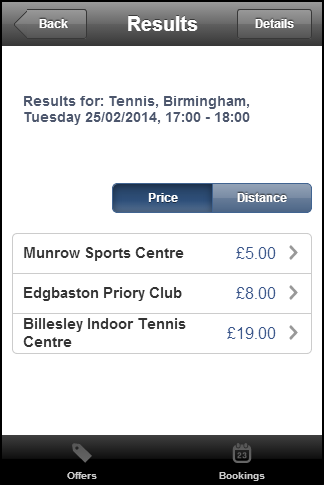
\includegraphics[width=\textwidth]{img/firstPrototypes/Pro3Results_1}
		\caption{Results displayed as a list}\label{fig:Pro3Results_1}
	\end{subfigure}%
	\qquad
	\begin{subfigure}[b]{0.45\textwidth}
		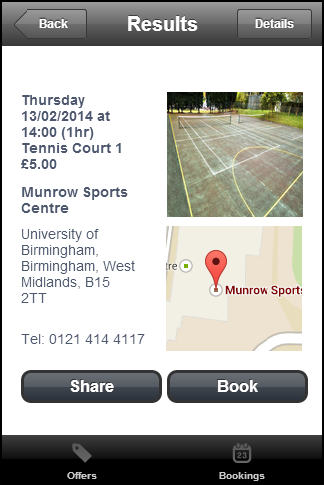
\includegraphics[width=\textwidth]{img/firstPrototypes/Pro3Results_2}
		\caption{Further information}\label{fig:Pro3Results_2}
	\end{subfigure}
	\caption{}\label{fig:Pro3Results}
\end{figure}

\marginpar{%
	\begin{overpic}[width=\marginparwidth]
		{img/firstPrototypes/Pro3Bookings_1}
	\end{overpic}
	\captionof{figure}{The bookings tab}\label{fig:Pro3Bookings_1}
}

\paragraph{Tab bar}

There are two tabs on the bar at the bottom of the screen;
\begin{itemize}
	\item `Offers' tab, shows available offers. A user could choose to use
		this to search for facilities by available offers.
	\item `Bookings' tab, users can keep track of their current and previous
		bookings.
\end{itemize}

\begin{figure}[htpb]
	\centering
	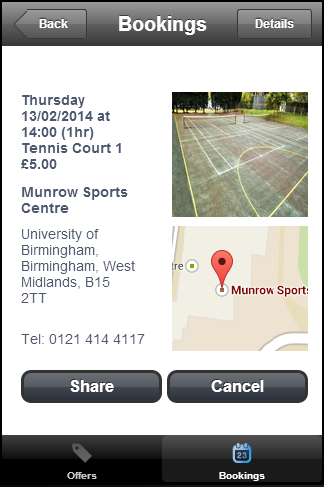
\includegraphics[width=0.45\linewidth]{img/firstPrototypes/Pro3Bookings_2}
	\caption{Further information is available}\label{fig:Pro3Bookings_2}
\end{figure}
% \marginpar{%
% 	\begin{overpic}[width=\marginparwidth]
% 		{img/firstPrototypes/Pro3Bookings_2}
% 	\end{overpic}
% 	\captionof{figure}{Further information is available}\label{fig:Pro3Bookings_2}
% }

\fullwidth%
\subsubsection{Evaluation}

\renewcommand{\arraystretch}{2}
% \begin{longtable}{@{\extracolsep{\fill}}p{0.3\linewidth} c p{0.6\linewidth}}
\begin{longtabu}{p{0.3\linewidth} c X}
	\toprule
	\textbf{Criteria} & \textbf{Rating} & \textbf{Comment}\\
	\midrule
	Visibility of system status & $+$ & There are only two states in this
	application, the search screen and the results page.\\

	Match between system and the real world & $+$ & Most other booking
	applications have a similar layout of a search page followed by a list
	of results (E.g.\ trainline, redspottedhanky). It should be easy for a
	user who is familiar with this format to use this design.\\

	User control and freedom & $+$ & `Back' button in the navigation bar
	allows the user to change elements of the search criteria.\\

	Consistency and standards & $+$ & Information is displayed in a similar
	way throughout the application, e.g.\  Bookings and Results both use
	lists and selecting a particular item in the list leads to a page with
	more specific information.\\

	Error prevention & $-$ & There is no way for a user to tell if they
	have made a mistake or where the errors are. A pop-up notification
	could supply this information when the user presses the `search'
	button.\\

	Recognition rather than recall & $+$ & Search criteria is displayed on
	the main page and in the results section.\\

	Flexibility and efficiency of use & $0$ & Novice users may not find this
	format easy-to-use without instructions.  Experienced users could also
	search for offers, or their current/previous bookings using the tab bar
	in addition to using the home screen. \\

	Aesthetic and minimalist design & $0$ & Keeping the search options on
	different pages prevents the home screen from becoming cluttered.
	However, presenting the results as a list may not be helpful for users
	who do not select a specific sport, date, time or location.\\

	Help users recognize, diagnose, and recover from errors & $-$ & There
	is no way for a user to tell if they have made an error. The only
	option available is to go `back' and change the search criteria.\\

	Help and documentation & $-$ & Currently there are no instructions
	available on how to use the application.\\
	\bottomrule
\end{longtabu}

\newpage

\renewcommand{\arraystretch}{2}
\begin{longtabu}{p{0.3\linewidth} c X}
	\toprule
	\textbf{Scenario} & \textbf{Rating} & \textbf{Comment}\\
	\midrule
	\multicolumn{3}{l}{\textbf{Elderly}}\\
	\midrule
	Searching for new sports in the area and notifying
	his wife of the booking. & $+$ & Howard can search using the location and
	distance criteria for searching for sports facilities locally. He can
	also send the details of his bookings to his wife by using the `share'
	button.\\

	Racquet sport with 4 friends on Friday & $0$ & Howard can select the
	individual sports from a list, there is no option at the moment for
	racquet sports. He can also choose a Friday, but wouldn't be able to
	bulk book for a regular session in-app.\\

	Swimming nearby with knee pain & $-$ & It isn't possible to search
	for facilities that have disabled access, this could be something to
	include in the `details' section and in the information pages of
	individual sports centres.\\

	\multicolumn{3}{l}{\textbf{Working}}\\
	\midrule
	Team sport on Friday including screen sharing with friends& $-$ & Janet
	can select individual sports like netball, football, etc.\  as there is
	no option for `team sports' and dates. She wouldn't be able to share
	all the results with her friends but could share individual bookings
	she selects.\\

	Change/cancel booking at late notice & $0$ & Using the `Bookings'
	tab, Janet could find her booking and cancel it using the `cancel'
	button, or use the information to contact the sports facility to change
	her booking.\\

	Outdoor sport early on Saturday & $+$ & Currently no quick filters
	for `outdoor' sports, Janet would have to go through the list of all
	possible sports and select those that she knows are outdoors.  Or it
	could be easier for Janet to select Saturday and mornings using the
	date and time sections and see what sports are available.\\

	\multicolumn{3}{l}{\textbf{Student}}\\
	\midrule
	Tennis court at specific times & $0$ & Jenny can select tennis only but
	may have to search a few times to find suitable slots for the different
	times she is free.\\

	Weekday evening session must be on clay & $0$ & Jenny can select the
	whole week and hours in the evenings in the `date' and `time' sections.
	She would have to check individual sports facilities to see the types
	of courts available.\\

	Weekly practice with friend with reminders & $0$ & There isn't a way
	for Jenny to book weekly sessions but could book one session a week and
	share the information with a friend using the `share' button.\\

	\multicolumn{3}{l}{\textbf{Child}}\\
	\midrule
	Outdoor sport close to home or on a bus route with coach & $0$ & It
	currently isn't possible to select `outdoor' sports but he could choose
	a variety of sports in the sports section and can sort by distance. It
	wouldn't be possible to know if the facilities are close to a bus route
	but could check with the facilities by contacting them.\\

	Booking several squash courts for after school tournament & $0$ & It
	isn't possible for Joe to book several courts at one time.

	Could have some kind of rating system to the location description on
	the bookings page and some way to search for highly rated locations.\\

	Looking for high quality tennis court & $0$ & It could be possible to
	include other users ratings of each facility and sort results by these
	ratings.\\
	\bottomrule
\end{longtabu}

\subsection{Conclusion}
\label{sub:flat_conclusion}

The design of the flat prototype is based on many other booking applications,
simply consisting of a `search' screen and a `results' screen, which should
make it easy to use for most people. This design allows users to input some
basic details which can help apply relevant offers to results. It also allows
users to keep track of their current and previous bookings.

Based on the results from the evaluation against heuristics, the design needs
to include error prevention and recovery, as well as help and documentation for
users who may not be familiar with mobile booking applications. The results
from the personas and scenarios show that although this design allows for
search criteria to not be specified by using the default selection of `any',
there is little flexibility in terms of sports selection, it wouldn’t be
possible to search on broader terms such as `outdoor', `racquet' or `team'.

Multiple bookings and group bookings also aren’t possible with this prototype,
though the `share' button makes it possible to share booking information with
others.

\restoregeometry%
